\section{Vector Spaces}
\label{sec:vector-spaces}

The arrows of Euclidean geometry are examples of a more general algebraic structure. This abstraction is essential because quantum states, functions, matrices, and solutions of differential equations can all behave like vectors.

\subsection{Axiomatic Structure}

A vector space $V$ over a field of scalars $\mathbb F$ is a set equipped with vector addition and scalar multiplication. These operations satisfy closure, associativity, commutativity of addition, additive identity and inverses, and the distributive and compatibility laws for scalar multiplication.

\begin{definition}
A subset $W\subseteq V$ is a subspace if it contains the zero vector and is closed under vector addition and scalar multiplication.
\end{definition}

\subsection{Examples Beyond Arrows}

Important vector spaces include
\begin{itemize}
\item ordered $n$-tuples $\mathbb R^n$ or $\mathbb C^n$;
\item polynomials of degree at most $n$;
\item matrices of fixed size;
\item continuous functions on an interval;
\item solutions of a homogeneous linear differential equation;
\item quantum state vectors in a Hilbert space.
\end{itemize}

For functions, addition and scalar multiplication are defined pointwise:
\[
(f+g)(x)=f(x)+g(x),
\qquad
(\lambda f)(x)=\lambda f(x).
\]

\begin{physical}
In quantum mechanics the word \emph{vector} usually does not mean an arrow in ordinary space. It means an element of a complex vector space whose linear combinations describe superposition.
\end{physical}

\begin{bookfigure}{Functions form vector spaces because pointwise sums and scalar multiples remain functions in the space.}
\begin{tikzpicture}[x=1cm,y=1cm]
\draw[book axis] (-.2,0)--(6.0,0) node[right] {$x$};
\draw[book axis] (0,-1.7)--(0,2.4) node[above] {$f(x)$};
\draw[book locus,samples=80,smooth,domain=0:5.6] plot (\x,{1.15*sin(70*\x)});
\draw[book accent,samples=80,smooth,domain=0:5.6] plot (\x,{.55*cos(110*\x)});
\draw[draw=visualcyan,line width=1.2pt,samples=80,smooth,domain=0:5.6] plot (\x,{1.15*sin(70*\x)+.55*cos(110*\x)});
\node[text=visualblue] at (4.8,1.85) {$f$}; \node[text=visualgold] at (5.15,-1.3) {$g$};
\node[text=visualcyan] at (2.1,1.85) {$f+g$};
\end{tikzpicture}

\label{fig:function-vector-space}
\end{bookfigure}

\booktopic{From Vector Spaces to Hilbert Spaces}

A vector space alone provides addition and scalar multiplication. Adding an inner product introduces lengths and angles; completeness then leads to a Hilbert space. These ideas will later support operators, eigenstates, orthogonality, and quantum measurement.

\begin{bookfigure}{Geometric arrows generalize to abstract vectors, Hilbert-space vectors, and quantum states.}
\begin{tikzpicture}[x=1cm,y=1cm]
\node[draw=visualblue,fill=softblue,rounded corners,minimum width=2.5cm,minimum height=1cm] (A) at (0,0) {geometric arrows};
\node[draw=visualcyan,fill=white,rounded corners,minimum width=2.5cm,minimum height=1cm] (B) at (3.7,0) {abstract vectors};
\node[draw=visualgold,fill=softgold,rounded corners,minimum width=2.5cm,minimum height=1cm] (C) at (7.4,0) {Hilbert space};
\node[draw=visualred,fill=softred,rounded corners,minimum width=2.5cm,minimum height=1cm] (D) at (11.1,0) {quantum states};
\draw[book transform] (A)--(B); \draw[book transform] (B)--(C); \draw[book transform] (C)--(D);
\node[below=7pt of A] {$\mathbb R^2,\mathbb R^3$}; \node[below=7pt of B] {functions, matrices};
\node[below=7pt of C] {inner product + completeness}; \node[below=7pt of D] {$|\psi\rangle$};
\end{tikzpicture}

\label{fig:hilbert-space-bridge}
\end{bookfigure}

\booktopic{Constructing an Orthonormal Basis}
Given independent vectors, the Gram--Schmidt process subtracts from each new vector the components already accounted for. For two vectors,
\[
\mathbf u_1=\mathbf v_1,\qquad
\mathbf u_2=\mathbf v_2-
\frac{\mathbf v_2\cdot\mathbf u_1}{\mathbf u_1\cdot\mathbf u_1}\mathbf u_1.
\]
Normalizing $\mathbf u_1$ and $\mathbf u_2$ produces orthonormal basis vectors.

\begin{bookfigure}{The Gram--Schmidt step removes the projection of $\mathbf v_2$ along $\mathbf u_1$, leaving an orthogonal direction.}
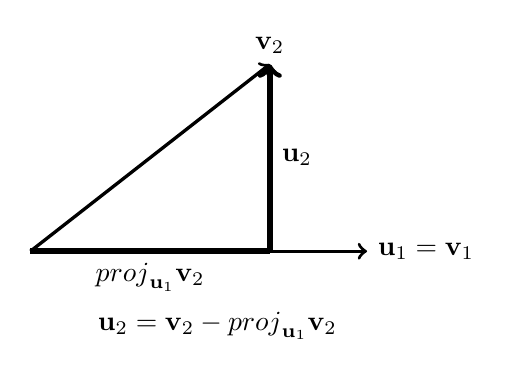
\begin{tikzpicture}[scale=0.95]
  \coordinate (O) at (0,0); \coordinate (U1) at (4.5,0); \coordinate (V2) at (3.2,2.5); \coordinate (P) at (3.2,0);
  \draw[->,very thick] (O)--(U1) node[right] {$\mathbf u_1=\mathbf v_1$};
  \draw[->,very thick] (O)--(V2) node[above] {$\mathbf v_2$};
  \draw[dashed] (V2)--(P);
  \draw[->,line width=2pt] (P)--(V2) node[midway,right] {$\mathbf u_2$};
  \draw[line width=2pt] (O)--(P) node[midway,below] {$\operatorname{proj}_{\mathbf u_1}\mathbf v_2$};
  \node[align=center] at (2.5,-1.0) {$\mathbf u_2=\mathbf v_2-\operatorname{proj}_{\mathbf u_1}\mathbf v_2$};
\end{tikzpicture}

\end{bookfigure}
